% Especificaciones del tamaño de letra, tamaño de hoja, márgenes, librerias, etc.
\documentclass[12pt, letterpaper]{article}
\usepackage[english]{babel}
\usepackage{fancyhdr}
\usepackage[utf8]{inputenc}
\usepackage[T1]{fontenc}
\usepackage{amsmath}
\usepackage{graphicx}
\usepackage{subcaption}
\usepackage[hidelinks]{hyperref}
\usepackage{url}
\usepackage{amssymb}
\usepackage{float}
\usepackage[margin=1in]{geometry}
\renewcommand{\baselinestretch}{1.5}

% Enlace Bibliografía
\usepackage{csquotes}
\usepackage[notes,backend=biber]{biblatex-chicago}
\addbibresource{referencias.bib}

% Titulo, autores, fecha.
\title{Tarea \#1: Diagrama Esfuerzo-Deformación}
\author{Carlos A. Vásquez Castañeda \and 1155057 \and Grupo 393}
\date{Septiembre 9, 2019}
\pagestyle{fancy}
\fancyhf{}
\rhead{Diseño de Elementos de Aeronaves}
\lhead{Tarea \#1}
\rfoot{\thepage}


% Inicio del documento
\begin{document}
\maketitle
La relación esfuerzo-deformación en un material dado es una característica importante del material. Para obtener el diagrama esfuerzo-deformación de un material, usualmente se lleva a cabo un ensayo o prueba de tensión sobre una probeta del material.

Los diagramas de esfuerzo-deformación de los materiales varían en forma considerable por lo que diferentes ensayosde tensión llevados a cabo sobre el mismo material pueden arrojar diferentes resultados, dependiendo de la temperatura de la probeta y de la velocidad de aplicación de la carga.

\begin{figure}[H]
	\centering
	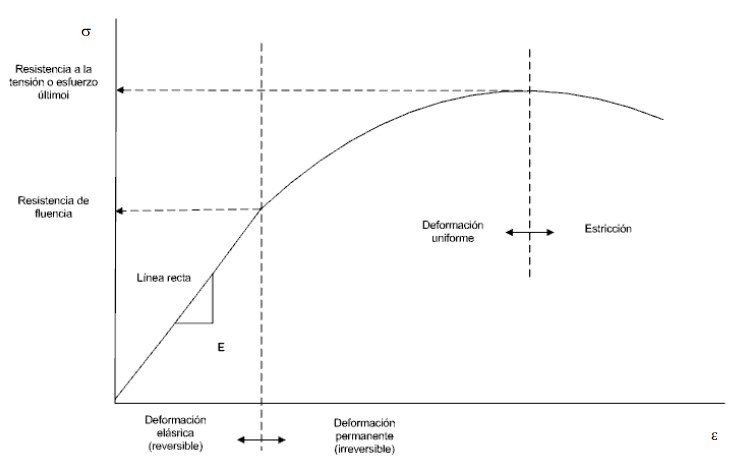
\includegraphics[width=0.9\textwidth]{1.png}
\end{figure}

En la figura es posible apreciar una gráfica esfuerzo-deformación. Cada segmento o punto en la curva recibe un nombre. El punto donde se encuentra la resistencia de fluencia realmente se encuentran dos puntos muy cercanos, el cual es el límite de proporcionalidad (donde se cumple la ley de Hooke) y justamente después del límite de proporcionalidad, la curva disminuye su pendiente y el material se deforma con muy poco o ningún aumento en la carga. Se dice que el material fluye o se deforma plásticamente en este punto, por lo que recibe el nombre de punto de fluencia. Posteriormente, la curva incrementa su pendiente y alcanza un valor máximo, el cual se conoce como la resistencia a la tensión o esfuerzo último que el material es capaz de soportar. Finalmente, después de este punto comienza la zona de estricción, donde la curva desciente hasta el púnto final que se conoce como el punto de fractura, y es donde la gráfica termina. Esto es un resumen general de la gráfica, a continuación analizaremos un poco más a fondo los datos que nos puede proporcionar.

El punto de fluencia también recibe otro nombre, la resistencia a la fluencia, cuyo valor de esfuerzo es que debe aplicarse sobre el material para iniciar su deformación permanente. Formalmente se define como el valor del esfuerzo que al ser aplicado al material produce una deformación permanente de 0.2\%.

La pendiente que está señalada en la figura que se forma en la zona elástica de la curva se conoce como módulo de elasticidad (E), la cual cumple la ley de Hooke ($\sigma = E\epsilon$). El módulo de elasticidad es una medida de la rigidez del material, lo cual quiere decir que se deforma elásticamente menos que otros materiales a los cuales se les aplica una carga determinada.

Otra medida importante es el módulo de resiliencia, el cual es el valor numérico del área bajo la curva dentro de la zona elástica. Éste representa la energía por unidad de volumen que el material absorbe cuando se deforma elásticamente.

La tenacidad es la energía por unidad de volumen que el material puede absorber antes de romperse. La tenacidad es numéricamente igual al área bajo la curva esfuerzo-deformación. No debe confundirse con el módulo de resiliencia, ya que la tenacidad es el área total debajo de la curva completa, a comparación del de resiliencia, que sólo se enfoca en el área de la zona elástica.
%%%%%  Bib
\renewcommand\refname{References}
\printbibliography
\end{document}
